\chapter{Experimental Evaluation}\label{ch:experimental_evaluation}



\section{Experimental Setup}


\subsection{Simulation}


% % Mention something about reproducibility, and that Docker image was created to easy this
% On the other hand, reproducibility is an underestimated issue in
% RL and not many researchers have tried to dig into the issue.
% It is not easy to reproduce results from many state-of-the-art
% papers since the implementation details were either missing
% or incomplete. The situation is even worse when coupled with
% the instability that RL algorithms currently suffer.


\subsection{Real}


\begin{figure}[ht]
    \centering
    % 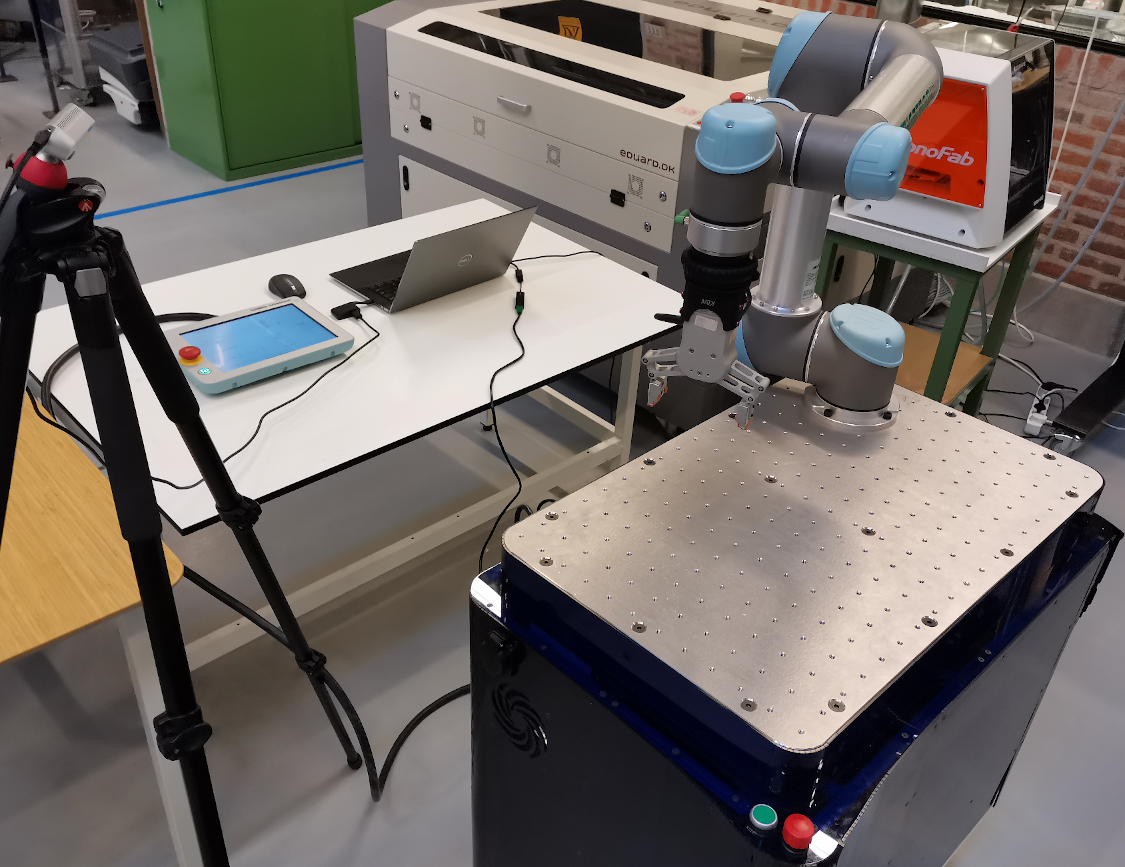
\includegraphics[width=0.666667\textwidth]{experimental_evaluation/real_setup.png}
    \caption{RealSense D435 camera and UR5 robot with RG2 gripper in a setup that is used to evaluate sim-to-real transfer.}
    \label{fig:real_setup}
\end{figure}

\begin{figure}[ht]
    \centering
    % 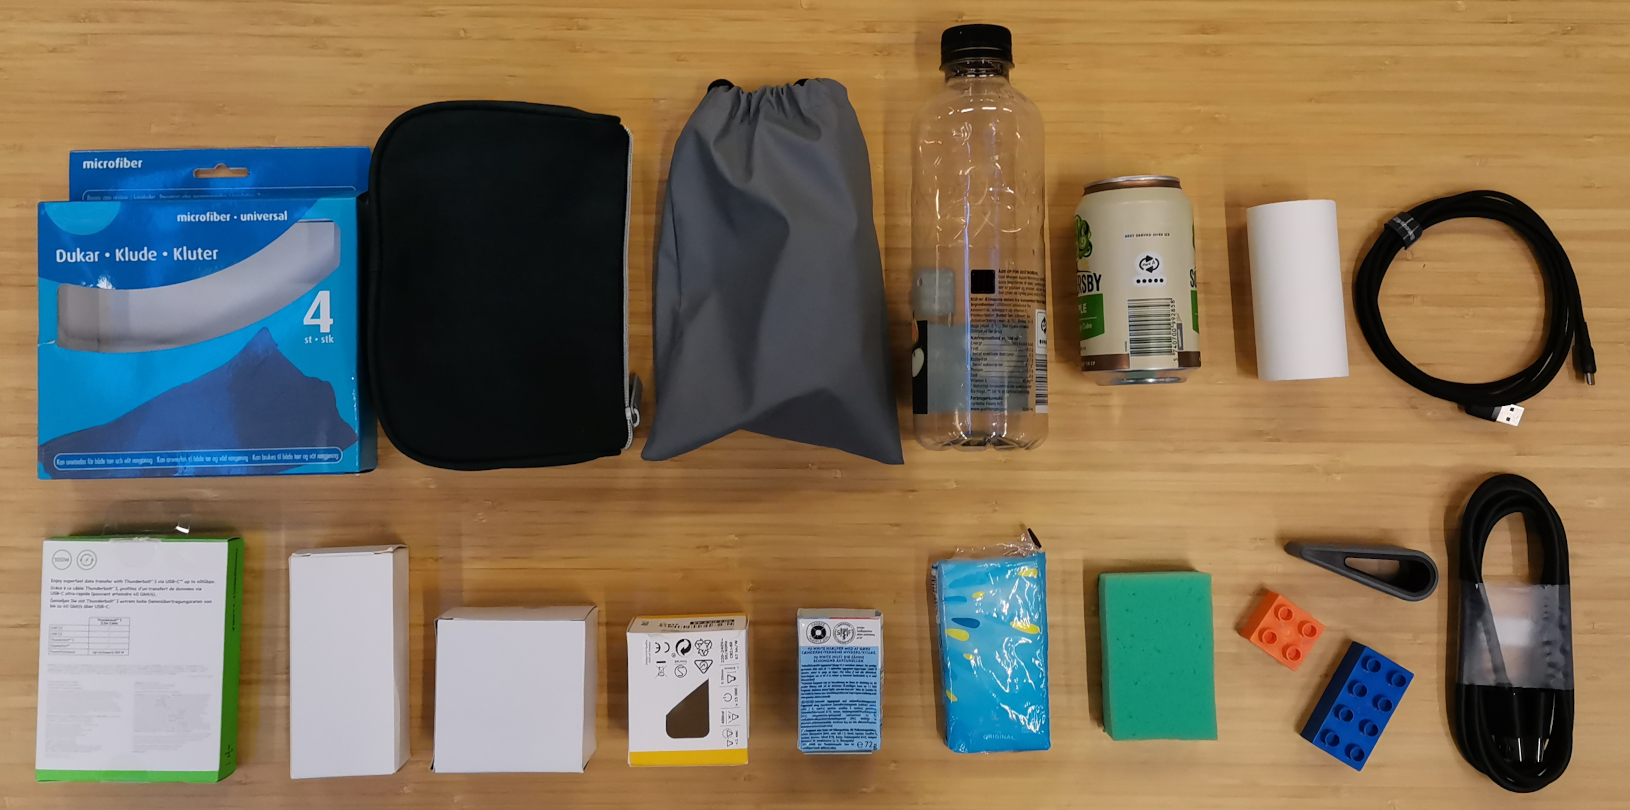
\includegraphics[width=0.77\textwidth]{experimental_evaluation/real_objects.png}
    \caption{A set of objects used during evaluation in real-world domain.}
    \label{fig:real_objects}
\end{figure}


% Test success rate for grasping from multiple views (on the same agent)
% Try mounting camera on robot to see what performance that gives (in simulation)

\section{Results}

\subsection{Comparison of Actor-Critic Algorithms}

\subsection{Comparison of 2D/2.5D/3D Feature Extraction}

\subsection{Invariance to Robot}

\subsection{Invariance to Camera Pose}

\subsection{Sim-to-Real Transfer}



\section{Ablation Studies}

\subsection{Curriculum}

\subsection{Demonstrations}

\subsection{Colour Features}

\subsection{Proprioceptive Observations}

\subsection{Sharing of Feature Extractor between Actor and Critics}

\subsection{Separate Feature Extractors for Stacked Observations}

